\documentclass[output=paper]{langscibook} 
\title{Linguistics as a science of structure}
\label{chap:nefdt}
\author{Ryan M. Nefdt \affiliation{University of the Western Cape}}

% \chapterDOI{} %will be filled in at production
%\setcounter{page}{0}
% \epigram{}

\abstract{Generative linguistics has rapidly changed during the course of a relatively short period. This has caused many to question its scientific status as a realist scientific theory \citep{Stokhof2011,Lappin2000}. In this chapter, I argue against this conclusion. Specifically, I claim that the mathematical foundations of the science present a different story below the surface. I agree with critics that due to the major shifts in theory over the past 80 years, linguistics is indeed opened up to the problem of pessimistic meta-induction or radical theory change. However, I further argue that a structural realist approach \citep{Ladyman1998,French2006} can save the field from this problem and at the same time capture its structural nature. I discuss particular historical instances of theory change in generative grammar as evidence for this interpretation and finally attempt to extend it beyond the generative tradition to encompass previous frameworks in linguistics.}
\begin{document}
\maketitle

\section{Introduction}
\label{sec:nefdt:intro}

The generativist revolution in linguistics started in the mid-1950s, inspired in large part by insights from mathematical logic and in particular proof theory. Since then, generative linguistics has become a dominant paradigm, with many connections to both the formal and natural sciences. At the centre of the newly established discipline was the syntactic or formal engine, the structures of which were revealed through modelling grammatical form. The generativist paradigm in linguistics initially relied heavily upon the proof-theoretic techniques introduced by Emil Post and other formal logicians to model the form language takes \citep{Tomalin2006, Pullum2011, Pullum2013}.\footnote{Here my focus will largely be on the formal history of generative syntax but I will make some comments on other aspects of linguistics along the way.} Yet despite these aforementioned formal beginnings, the generative theory of linguistics has changed its commitments quite drastically over the intervening years, eschewing among other things formalization, cognitive science for evolutionary biology, derivations for constraints, rules for schemata, phrase structure for cyclic phases of the merge operation and other theoretical choices.  

Given significant theory change, the fecundity of the enterprise and its so-called discoveries are inevitably called into question \citep{Stokhof2011,Lappin2000,Jackendoff2002}. A related, more ontological, question is, if the grammars of linguistics are scientific theories (as Chomsky and others have insisted over the years), then what are the objects being explained by these grammars? The former question has received little attention as compared to the latter.\footnote {See \cite{Chomsky1986} for the received psychological view on the ontology of linguistics, \cite{Katz1991} for a Platonist interpretation, \cite{Devitt2006} for a non-psychological physicalist view, and \cite{Stainton2014} for a mixture of all the above. See \cite{Nefdt:2018} for an alternative mixture of these views.} I will not directly add to the ontological debate here, but I do hope to draw some needed attention to the question of theory change in linguistics. 

Thus, in this chapter, I argue that linguistics as a science faces the problem of pessimistic meta-induction, more generally discussed in the philosophy of the hard science such as physics. In addition, I claim that the focus on the ontology of linguistic objects, such as words, phrases, sentences etc. belies the formal nature of the field, which is at base a structural undertaking. Both of these claims, I argue, lead to the interpretation of linguistics in terms of ontic structural realism in the philosophy of science \citep{Ladyman1998, French2006}. Thus, to be realist in this sense is to accept the existence of linguistic structures (not their content) defined internally through the operations of the grammars, and what remains relatively stable across various theoretical shifts in the generative paradigm, from Standard Theory (1957--1980) to the Minimalist Program (1995--present), are the formal structures so defined. 

The chapter is separated into three parts. In the first part, I discuss the various theoretical changes which the generative linguistic tradition has undergone since its inception in the late 1950s. For instance, the move from rewriting systems with transformations to X-bar representation \citep{Chomsky1970} with theta roles to the current single movement operator Merge contained only by constraints. Despite appearances, I hope to show that the structure of these representations has remained relatively constant. In the second part, I discuss structural realism in the philosophy of science more generally and why it might serve as an illuminating foundation for linguistics. Linguistics here is interpreted structurally without recourse to the independent existence of individual objects or contents in that structure (along the lines of \citealt{Shapiro1997} for mathematics). In other words, there are no phrases, clauses or sentences outside the overarching linguistic structure described by the grammar. Lastly, I briefly show that once a structural realist framework is adopted for the study of language, connections and continuity beyond current generative paradigms become apparent.  

\section{Theory change in generative linguistics}
\label{sec:nefdt:theorychange}

The history of science has seen a number of radical theory changes, from Newtonian to Relativistic physics, from Euclidean to Riemannian geometry as a characterization of physical space, from phlogiston theory to Lavoiser's oxygen theory, among many others. In the course of such changes, one might easily dismiss the old theory as simply false. However, as \cite{Laudan1981} convincingly showed, there is a deeper issue looming in the passage of time, namely what has become known as pessimistic meta-induction (\textsc{pmi}). \textsc{pmi} can be defined as follows for present purposes. 

\begin{description}
\item[\textsc{pmi}]: If all (most) previous scientific theories have been shown to be false, then what reason do we have to believe in the truth of current theories?
\end{description}

The problem with radical theory change is that it causes serious tension for any realist theory of science, which aims to hold to the truth or approximate truth of current theories. Of course, false theories can be responsible for true ones through some sort of trial-and-error process. But the idea that our best current theories are of mere instrumental value for later truth is hard to accept.\footnote{There are such instrumentalist theories on the market. Van Fraassen's (\citeyear{vanFraasen1980}) constructive empiricism is one prominent example. A general problem for such views is that they tend to make miraculous the explanatory and predictive successes of scientific theory.} Furthermore, at no point will certainty naturally force itself upon us, especially since success is not a guarantee of truth (e.g. classical mechanics is still a useful tool for modelling physical phenomena). \textsc{pmi} has an ontological component as well. When theories do change, they often propose distinct and incompatible entities in their respective ontologies. Consider the move from phlogiston theory to oxygen theory. In fact, the term ``phlogiston'' has become synonymous with a theoretical term which does not refer to anything. Essentially, the ontological status of the objects of the theories are rendered problematic when radical theory change occurs, which prompts a challenge again to the realist. ``[I]f she can't establish the metaphysical status of the objects at the heart of her ontology, how can she adopt a realist attitude towards them?'' \citep[165]{French2011}.

Linguistics, too, has seen its fair share of radical shifts in theory and perspective over the past few decades. In fact, the early generative tradition of \cite{Chomsky1957} had a more formal mathematical outlook. Drawing inspiration from the work of Emil Post on canonical production systems, which are distinctively proof-theoretic devices in which symbols are manipulated via rules of inference in order to arrive at particular formulas (not unlike natural deduction systems), linguistics approached language from a more syntactic perspective.\footnote{For a thorough discussion of the influence of Post on generative grammar, see \cite{Pullum2011} and \cite{Lobina2017}.} This was due in part to two assumptions, namely (1) that syntax is autonomous from semantics, phonology etc. and (2) that syntax or the form of language is more amenable, than say semantic meaning, to precise mathematical elucidation. However, it must be added that as early as \textit{Syntactic Structures} (1) had often been advanced as a necessary condition for progress in semantics.\footnote{I thank Michael Kac for emphasizing this point to me.} Mathematical models of this sort would be a key tool in early generative linguistic analysis. Chomsky states the formal position in the following way at the time:\footnote{I attempt to follow \cite{Pullum2007} throughout in slaloming my way through the minefield of the distinctions between ``formalization'', ``formal'', and ``Formalism''. The senses expressed here are related to ``formal'' as a term used for systems which abstract over meaning and ``formalization'' as a tool for converting statements of theory into precise mathematical representations. Early generative grammar can be seen as a theory which aimed to achieve both distinct goals.} 

\begin{quote}
Precisely constructed models for linguistic structure can play an important role, both positive and negative, in the process of discovery itself. By pushing a precise but inadequate formulation to an unacceptable conclusion, we can often expose the exact source of this inadequacy and, consequently, gain a deeper understanding of the linguistic data. More positively, a formalized theory may automatically provide solutions for many problems other than those for which it was explicitly designed. \citep[5]{Chomsky1957}
\end{quote}

He goes on to chastise linguists who are sceptical of formal methods. However, as we shall see, the course of linguistic theory saw a decrease in formalization and an increased resistance to it (partly inspired by Chomsky's later views). In fact, a generative grammar in the early stages was expressly noncommittal on ontological questions: ``Each such grammar is simply a description of a certain set of utterances, namely, those which it generates'' \citep[48]{Chomsky1957}. By the 1960s, grammars were reconceived as tools for revealing linguistic competence or the idealized mental states of language users. With mentalism, linguistics looked towards sciences such as psychology, physics, and biology for methodological guidance as opposed to logic and mathematics as it did before. As \cite[167]{Cowie1999} states of the time after \emph{Aspects}, Chomsky ``seemed also to have found a new methodology for the psychological study of language and created a new job description for linguists''. The psychological interpretation of linguistic theory held sway until the 1990s, when the biolinguistic program emerged as yet another new way of theorizing about language. The \emph{Minimalist Program} (\citeyear{Chomsky1995MP}) pushed the field towards understanding language as a ``natural object'', in which questions of its optimal design and evolution take centre-stage.\footnote{Of course, matters are rarely this simple or clear. For instance, \cite{Bickerton2014} stresses that the peculiarity of the situation in linguistics is that the field at present still contains scholars working in various versions of the generative programme concurrently.}

Each new foundation distanced itself from the methodology of its predecessor, postulated different objects and advocated different ends. Thus, \textsc{pmi} takes on special significance for linguistics and an answer to the puzzles it presents become especially peremptory in this light. In the following sections, I will focus on some specific cases of the methodological changes which underlie the picture sketched above. 


\section{From phrases to phases}
\label{sec:nefdt:phrasephase}

In this section, I aim to provide a story of the mathematical formalisms employed in the service of an ever-changing landscape of theory in linguistics. I will not, however, directly discuss theoretical postulates such as Universal Grammar or modularity etc., which lie outside the scope of the present purview.

The early generative approach had a particular notion of a language and accompanying grammar at its core. On this view, a language $L$ is modelled on a formal language which is a set of strings characterizable in terms of a grammar $G$ or a rule-bound device responsible for generating well-formed formulas (i.e. grammatical expressions). In \textsc{lslt}, \cite[5]{Chomsky1975} writes of a language that it is ``a set (in general infinite) of finite strings of symbols drawn from a finite `alphabet'\thinspace''. In formal language theory (\textsc{flt}) (which took inspiration from this period), assuming a start symbol $S$, set of terminals (words) $T$, nonterminals $NT$ (syntactic categories) and production rules $R$, we can define a grammar in the following way:

\begin{quote}
$G$ will be said to \emph{generate} a string $w$ consisting of symbols from $\Sigma$ if and only if it is possible to start with $S$ and produce $w$ through some finite sequence of rule applications. The sequence of modified strings that proceeds from $S$ to $w$ is called a \emph{derivation} of $w$. The set of all strings that $G$ can generate is called the \emph{language} of $G$, and is notated $\mathcal{L}(G)$ \citep[1957]{Jager2012}. 
\end{quote}

In \cite{Chomsky1956}, natural languages were shown to be beyond the scope of languages with production rules such as $A\rightarrow a,$ $A\rightarrow aB$
or $A\rightarrow\varepsilon$ ($\varepsilon$ is the empty string)
such that $A,B\in NT$ and $a\in T$ (i.e. regular languages).\footnote{One issue is that regular grammars cannot capture centre embeddings such as \emph{The boy the girl loved left}.} This result lead to the advent of phrase-structure or context-free grammars with production rules of the following sort: either $S\rightarrow ab$ or $S\rightarrow aSb$ (read the arrow as ``replace with'' or rewrite). These grammars can handle recursive structures and contain the regular languages as a proper subset. For many years, phrase-structure grammars were the standard way of describing linguistic phenomena. Essentially, phrase structure grammars are rewriting systems in which symbols are replaced with others such as $S\rightarrow NP, VP$ or $NP\rightarrow det, N'$. As \citet[897]{Freidin2012} notes, ``phrase structure rules are based on a top-down analysis where a sentence is divided into its major constituent parts and then these parts are further divided into constituents, and so on until we reach lexical items''. There are a number of equivalent means of representing the structure of sentences in this way. The most common is \emph{via} hierarchical diagrams, shown below. 

\begin{enumerate}
\item \leavevmode\vadjust{\vspace{-\baselineskip}}\newline
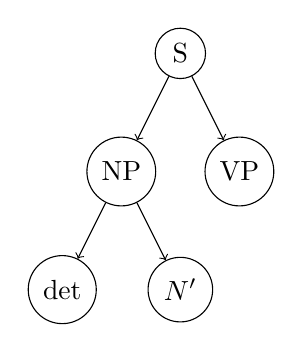
\begin{tikzpicture}[nodes={draw, circle}, ->]
 
   \node{S}
    child { node {NP} 
        child { node {det} }
        child { node {$N'$} }
    }
    child { node {VP} };
 
\end{tikzpicture}
\end{enumerate}

Alternatively one can capture the same information as:
\begin{enumerate}
    \item[2.] $[_S[_{NP}[_{det}][_{N'}]][_{VP}]]$
\end{enumerate} 

This basic structure, however, proved inadequate as a means of capturing the structure of passives and certain verbal auxiliary constructions as shown originally in \cite{Postal1964}.\footnote{This picture of the trajectory of the grammatical formalization is necessarily sketchy. A fuller story would include formal results such as \cite{Shieber1985}, which showed from the cross serial dependencies of Swiss-German that natural language syntax cannot be captured by a context-free grammar.} Transformations were meant to buttress the phrase structure system in order to bridge this gap in explanation. Transformation rules operate on the output of the phrase structure rules and create a derived structure, as in (3) below for passivization.

\begin{enumerate}
    \item[3.] $NP_1$ V $NP_2$ $\rightarrow$ $NP_2$ be-en (\textsc{aux}) V $NP_1$
\end{enumerate} 

The combined expressive power of phrase structure and transformations proved very productive in characterizing myriad linguistic structures. This productivity, with its increased complexity, however, came at a cost to learnability. ``[I]f a linguistic theory is to be explanatorily adequate it must not merely describe the facts, but must do so in a way that \emph{explains} how humans are able to learn languages'' \citep[15]{Ludlow2011}. The move to more generality led in part to the Extended Standard Theory and the X-bar schema.   

Since the continued proliferation of transformations and phrase structure rules was considered to be cognitively unrealistic, linguistic structures needed more sparse mathematical representation. Although, as \cite[24]{Bickerton2014} states, ``rule proliferation and `ordering paradoxes' were only two of a number of problems that led to the eventual replacement of the Standard Theory''.\footnote{``Ordering paradoxes'' here refer to the situation in which there are equally valid reasons for orderings from X to Y and Y to X despite the grammar requiring a particular order to pertain.}

There was also a theoretical push for more general structure from the Universal Grammar (\textsc{ug}) postulate assumed to be the natural linguistic endowment of every language user. \textsc{ug} needed to contain more general rule schemata in order to account for the diversity of constructions across the world's languages. This structural agenda dovetailed well with the Principles and Parameters (\textsc{p\&p}) framework, which posited that the architecture of the language faculty constituted a limited number of universal principles constrained by individual parametric settings, where ``parameters'' were roughly the set of possible variations of a given structure. For instance, some languages, such as English, require a mandatory \textsc{np}/\textsc{dp} in the subject position of sentences, whereas in pro-drop languages, such as Spanish, empty categories can do the job. 

\begin{enumerate}
    \item[4.] It is raining.
    \item[5.] Llueve.
\end{enumerate}

These kinds of differences could be expressed in the language of parametric settings. The so-called Extended Projection Principle might be universal, but certain languages can contain distinct parameters with relation to it (such as fulfilling it with a null determiner). In other words, a child in the process of acquiring her first language can ``set'' the parameter based on the available linguistic environment in which she finds herself, like the flicking of a switch. Furthermore, this kind of structural picture is represented well in the X-bar schema \citep{Jackendoff1977}, which contains only three basic rules. There is (1) a specifier, (2) an adjunct, and (3) a complement rule. The specifier rule is given below (where $X'$ is a head-variable and $XP$ and $YP$ are arbitrary phrasal categories determined by that head).
\begin{itemize}
\item[6.] Specifier rule: $XP\rightarrow (Spec)X'$ or $XP\rightarrow X'(YP)$
\end{itemize}

Or equivalently:

\Tree [.XP [.specifier ] [.X' [.X ] [.complement ] ] ] 
\smallskip

A vast amount of linguistic structure can be modelled by means of this formalism. In fact, X-bar theory overgenerates structural descriptions (which need to be reined in by various constraints). But the underlying idea is that our mental competence is more likely to contain generalized rule schemata such as those above than individual phrase structure rules and countless transformations for each natural language. In a sense, X-bar merely smooths over the individual hierarchical structures of before and homes in on a more abstract structural representation for language. As Poole mentions:

\begin{quote}
[W]e discovered that your language faculty appears to structure phrases into three levels: the maximal projections or $XP$ level, the intermediate $X'$ level, and the head or $X^{\circ}$. \citep[50]{Poole2002}
\end{quote}

These rules subsume the previous \textit{ad hoc} phrase structure rules. Importantly, however, the representation only allows for binary rules (unlike the possible n-ary branches of phrase structure trees). \cite{Freidin2012} further claims that X-bar theory represented a shift from top-down to bottom-up analysis, despite being formulated in a top-down manner a decade after its inception. Here, the idea is that the rules stated above are projections from lexical items to syntactic category labels, not the other way around. 

Unfortunately, history has a way of repeating itself. Where in the previous instantiation of generative grammar, the proliferation of transformations became unwieldy, parameters would soon see a similar fate befall its fecundity. Briefly, \textsc{ug} was assumed to be extremely rich during this period: ``the available devices must be rich and diverse enough to deal with the phenomena exhibited in the possible human languages'' \citep[55]{Chomsky1986}. However, what was innate and what was learned or set by experience relied in part on a distinction between ``core'' grammar and ``periphery'', which was never explicitly provided by the theory (see \citealt{Pullum1983} and \citealt{Culicover2011} for discussion). Although formally all previous transformations were reduced to the ``move alpha'' operation, the multiplication of parameters took similar shape to its transformational predecessor. Newmeyer describes this period as one of instability and confusion:

\begin{quote}
In the worst-case scenario, an investigation of the properties of hundreds of languages around the world deepens the amount of parametric variation postulated among languages, and the number of possible settings for each parameter could grow so large that the term \textquoteleft{}parameter' could end up being nothing more than jargon for language-particular rule. \citep[64]{Newmeyer1996}
\end{quote}

In addition, these parameters seemed to force the violation of the binary requirement set by the X-bar formalism and with it the cognitive plausibility transiently acquired after the Standard Theory. There needed to be a better way of capturing the movement toward simplifying the grammatical representation and theory of natural language syntax. This and other theoretical motivations led to the Minimalist Program \citep{Chomsky1995MP}, which pushed the new biolinguistic agenda and a call for further simplicity. 

As mentioned in \sectref{sec:nefdt:theorychange}, the question of the evolution of language reset the agenda in theoretical linguistics at this time. The grammatical formalisms assumed to underlie the cognitive aspects of linguistic competence were forced to change with this new perspective, with the result that many of the advances made by the \textsc{p\&p} and Government and Binding \citep{Chomsky1981} theories needed to be abandoned. The rationale was something of the following sort:

\begin{quote}
Evolutionarily speaking, it is hard to explain the appearance of highly detailed, highly language-specific mental mechanisms. Conversely, it would be much easier to explain language's evolution in humans if it were composed of just a few very simple mechanisms \citep[175]{Johnson2015}.
\end{quote}

The Merge operation represented the goal of reducing structure to these simple mechanisms. In the Standard and Extended theories, grammars followed the structures set by the proof theory of the early twentieth century (see above), which often resulted in grammars ``of roughly the order of complexity of what is to be explained'' \citep[233]{Chomsky1995}. In the Minimalist programme, this apparatus was reduced to a simple set-theoretic operation which takes two syntactic objects and creates a labelled output of their composition (the label to be determined by the features of the objects thereby replacing the projection from heads of X-bar theory).\footnote{Technically, as \citet[307]{Langendoen:2003} notes, ``Merge is not a single operation, but a family of operations. To belong to the merge family, an operation must be able to yield an infinite set of objects from a finite basis''. However, by this definition, the phrase structure rules with recursive components would be invited to Thanksgiving dinner. The structural similarities of various versions of this infinity requirement on grammars will be discussed in the next section.} The formulation is given below:

\begin{enumerate}
    \item[7.] Merge$(\alpha,\beta)$ = $\{\gamma,\{\alpha,\beta\}\}$
\end{enumerate}
Or again, equivalently:

\Tree [.$\gamma$ [ [.$\alpha$ ] [.$\beta$ ]]]

The above is an example of external set merge (where $\gamma$ is a label projected from one of the elements). Internal merge accounts for recursive structures since it applies to its own output (as in if $\beta$ is already contained in $\alpha$). Consider the following sentence. 

\begin{enumerate}
    \item[8.] The driver will speed recklessly.
\end{enumerate}

In a bottom-up fashion, \emph{speed} and \emph{recklessly} will merge to form a \textsc{vp}, and thereafter this union will merge with the auxiliary \emph{will} to form a \textsc{tp} or Tense Phrase. Merge will independently take \emph{the} and \emph{driver} and create an \textsc{np} which will merge to form the final \textsc{tp} to deliver (8) above (the T is the label projected for the entire syntactic object). Importantly for the proposal I will present, ``[t]his last step merges two independent phrases in essentially the same way that generalized transformations operated in the earliest transformational grammars'' \citep[911]{Freidin2012}.\footnote{Of course, the practice of taking ideas or insights in disguised form from early frameworks was not uncommon. For instance, the binding theory of Government and Binding is very close (if not identical) to principles governing anaphora (like
the Ross-Langacker constraints) that were first articulated in the
1960s. Similarly, the trace theory of movement is closely
tied to the earlier idea of global derivational constraints. I thank Michael Kac for drawing my attention to these cases.} Thus, although the phrase structure rules had been replaced by the less complex merge operation with \emph{phases}, which are cyclic stages applying to the innermost constituents of the entire process \citep{Chomsky2008}, there is a similar structure to the derivation. 

Of course, unlike the top-down analysis of early generative grammar, Merge operates from lexical items in the opposite direction (Merge and the ``lexical array'' constituting ``narrow syntax'', see \citealt{Langendoen:2003}). However, as \citet[84]{Lobina2017} cautions, ``talk of top-down and bottom-up derivations is clearly metaphorical''.\footnote{Compare this metaphorical language to a similar caution in \cite[496]{Pullum2013}, ``[t]he fact that derivational steps come in a sequence has encouraged the practice of talking about them in procedural terms. Although this is merely a metaphor, it has come to have a firm grip on linguists thinking about syntax''.} It might add something in appreciating the flavour of the computational process at hand, but often the overall structural picture is unchanged by such parlance. 

Let this serve as an account, albeit incomplete, of some of the formal and theoretical changes of generative grammar over the 60-year period since its inception. Below, I will draw on the picture developed here to argue for the structural continuity of linguistics despite the theoretical shifts the overarching theory might have taken during this time.

\section{Structural realism and linguistics}
\label{sec:nefdt:structuralrealism}

The previous two sections showed a theoretical landscape in flux with each new stage abandoning the commitments of its predecessor. In such a scenario, \textsc{pmi} takes on a strong force. Not only this, but as mentioned before, the situation in linguistics is unique, since practitioners of each epoch of the theory can still be found working within the remit of their chosen formalism. In \sectref{sec:nefdt:theorychange}, I described some of the theoretical shifts in the generative paradigm since the 1950s. In \sectref{sec:nefdt:phrasephase}, I described the underlying mathematical formalisms utilized in service of the changing theory at each junction. In this section, I want to use a structural realist analysis of linguistics to show that despite the former, the structures of the latter remained relatively constant or at least commensurable. 

What is structural realism? One way of thinking of it is as the ``best of both worlds'' strategy for dealing with \textsc{pmi}. Realists, as we have seen, have trouble holding on to the objects of their theories once better theories come along. Anti-realists, on the other hand, have trouble accounting for the unparalleled predictive and explanatory success of theories (whose objects do not refer to objects in reality). Structural realism offers a conciliatory intermediary position between these choices. Ladyman describes the position as follows:

\begin{quote}
Rather we should adopt the structural realist emphasis on the mathematical or structural content of our theories. Since there is (says Worrall) retention of structure across theory change, structural realism both (a) avoids the force of the pessimistic meta-induction (by not committing us to belief in the theory's description of the furniture of the world), and (b) does not make the success of science […] seem miraculous (by committing us to the claim that the theory's structure, over and above its empirical content, describes the world). \citep[410]{Ladyman1998}
\end{quote}

There are two versions of structural realism in the philosophy of science. The first, initially proposed by \cite{Worall1989}, is epistemic in nature. The second, championed by \cite{French2003}, is an ontological proposal. The former involves the idea that all we can \emph{know} is structure, while the latter is a claim about all \emph{there is}. In other words, what is preserved across theory change is a kind of structure posited by the underlying equations, laws, models or other mathematical representations of the theories. Part of the reason I opt here for ontic structural realism is that there is an ontological component to \textsc{pmi}, as mentioned before. Thus, we are not only interested in what is communicated or epistemically accessible between different theories over time but what these theories say exists as well. The ontological answer to \textsc{pmi} is therefore that if we cannot be realists about the objects of our scientific theories, we can be realists about the structures that they posit.\footnote{At this point, one can glean how such a picture might enter into the debate concerning the ontological foundations of linguistics mentioned earlier. Unlike Platonists, who claim among other things that languages are individual abstract objects like sets, or mentalists, who claim they are psychological or internal states of the brain, a structuralist could argue that languages are complex structures in part identified by abstract rules and physical properties. See \cite{Nefdt:2018} for precisely such a view.}  

From here, it is not hard to see what the argument of the present section is going to be, namely that different generations of generative grammar display structural continuity notwithstanding variation in theoretical commitment. The means by which we can appreciate this continuity is by considering features of the mathematical representations employed during the course of history which could affect my proposed analysis. Moss has a similar idea when he discusses the contribution made by mathematical models to linguistic theory. 

\begin{quote}
[L]anguage comes to us without any evident structure. It is up to theoreticians to propose whatever structures they think are useful […] Mathematical models are the primary way that scientists in any field get at structure. \citep[534]{Moss2012}
\end{quote}

In the previous section, I told a story about how the proof-theoretic grammars of the Standard Theory were transformed into X-bar representations, which eventually led to the Merge operation in Minimalism. However, a remarkable fact about the structural descriptions generated by these various formalisms is that they share a number of essential features: (1) they generate the same sets of sentences (also called ``weak generative capacity''),\footnote{In fact, these equivalences go beyond the generative grammars.  Minimalist Syntax (or the \citealt{Stabler1997} version), Phrase-Structure grammars, Tree-substitution grammars, Head-Driven Phrase Structure grammars (\textsc{hpsg}), and Dependency grammars have been shown to share weak generative capacity. See \cite{Monnich2007}.} (2) they take a finite input and generate an infinite output, and (3) they can be represented hierarchically through tree structures (not to mention actual structural similarities such as the way in which Merge joins two independent clauses and the way it was proposed in early transformational grammar). None of these latter properties are trivial. For instance, dependency grammars can be shown to be weakly equivalent to phrase structure grammars but are represented by means of flat structures. Model-theoretic grammars, such as Head-Driven Phrase Structure Grammar, are usually hierarchically represented and can generate the same sets of sentences but do not have any cardinality commitments. 

It is important to note that there were a number of formal shifts present in the transitions from transformational grammars to Merge which might challenge the framework put forward here. I have already mentioned the top-down to bottom-up change and argued that, from a structural point of view, this is largely a metaphorical distinction. There is, however, another property of formal representations of syntax which also shifted from early to later generative grammar, namely from derivational approaches to representational or constraint-based ones. Simply put, derivational approaches follow the proof-theoretic model discussed earlier, where given a certain finite input and a certain set of rules, a particular structured output is generated. Constraint-based formalisms operate differently. Rather than \textquoteleft deriving' an expression as output from a rule-bound grammar, these formalisms define certain conditions upon expression-hood or what counts as a grammatical sentence of the language. Chomsky discusses this shift in thought in the following way:

\begin{quote}
If the question is real, and subject to inquiry, then the [strong minimalist thesis] might turn out to be an even more radical break from the tradition than [the principles-and-parameters model] seemed to be. Not only does it abandon traditional conceptions of ``rule of grammar'' and ``grammatical construction'' that were carried over in some form into generative grammar, but it may also set the stage for asking novel questions that have no real counterpart in the earlier study of language. \citep[92]{Chomsky2000}
\end{quote}

Indeed, with the Minimalist agenda and the Merge operation, more constraint-based grammar formalisms were embraced and adopted. This latter approach involves a different idea of ``rule of grammar'' and indeed ``grammar construction''. The formal difference can be understood in terms of how each type of formalism answers the so-called ``membership problem''. Decidability is an important aspect of formal language theory. Given a string $w$ and a formal language $\mathcal{L}(G)$, there is a finite procedure for deciding whether $w\in\mathcal{L}(G),$ i.e. a Turing machine which outputs {}``yes'' or {}``no'' in finite time. In other words, a language $\mathcal{L}(G)$ is decidable if
$G$ is a decidable grammar. This is called the membership problem. What determines membership in a traditional proof-theoretic grammar is whether or not that string can be generated from the start symbol $S$ and the production rules $R$. In other words, whether that string is recursively enumerable in that language (set of strings). What determines membership in a constraint-based grammar is whether the expression fulfils the constraints set by the grammar (which are like axioms of the system). ``An \textsc{mts} [model-theoretic syntax] grammar does not recursively define a set of expressions; it merely states necessary conditions on the syntactic structures of individual expressions'' \citep[19]{Pullum2001}. As mentioned above, Generalized Phrase Structure Grammar and Head-Driven Phrase Structure Grammar are formalisms of the latter variety. While phrase structure grammars can be found in the average syntax textbook, tree-adjoining grammars fall within the former camp.

The interesting fact for our purposes is that Merge and Minimalism represent the fruition of the gradual shift from derivational grammars to constraint-based ones. However, \cite{Chomsky2000} does not initially put much stock in this formal transition, despite the strong statement quoted above. He considers the old derivational or ``step-by-step procedure for constructing Exps'' approach and the ``direct definition […] where E is an expression of L iff …E…, where …-… is some condition on E'' approach to be ``mostly intertranslatable'' \citep[99]{Chomsky2000}.\footnote{He goes on to ``suspect'' that the adoption of the derivational approach is more than expository and might indeed be ``correct''.} Here he holds these formalism types to have few empirical differences.

From a mathematical point of view, the same formal languages and the structures of which they are composed are definable through both generative enumerative and model-theoretic means. Traditionally, the formal languages of the Chomsky Hierarchy were defined in terms of the kinds of grammars specified at the beginning of the previous section. However, there are other ways of demarcating the formal languages without recourse to generative grammars. For instance, they can be defined according to monadic second-order logic in the model-theoretic way. \cite{Buchi1960} showed that a set of strings forms a regular language if and only if it can be defined in the weak monadic second-order theory of the natural numbers with a successor. \cite{Thatcher1968} then showed that context-free languages ``were all and only the sets of strings forming the yield of sets of finite trees definable in the weak monadic second-order theory of multiple successors'' \citep[1117]{Rogers1998b}.

The point is that the same structures can be characterized by means of either proof-theoretic or model-theoretic techniques. Thus, the move from the former to the latter should not be seen as a hazard to the structural realist account of linguistic theory I am proffering here.\footnote{In terms of the nature of structural properties themselves, there are at least two possible ways in which to identify a structural property in the literature, one in terms of direct \textit{definability} and another \emph{via} a particular notion of \textit{invariance} across structures. See \cite{Korbmacher2017} for a formal comparison between these two options and \cite{Johnson2015} for an application of the latter to linguistic theory.} 

\section{In search of lost paradigms}
\label{sec:nefdt:lostparadigms}

The picture painted above is perhaps rather parochial. I consider theoretical shifts within the generative paradigm exclusively as a means of demonstrating the advantages of a structural realist interpretation of the science. There were a number of reasons for this narrow focus. One reason was that, with the centrality of syntax in the early generative tradition, the idea of form over content naturally led to a structural picture. Another reason was related to various criticisms levelled against the theoretical changes and the threat of \textsc{pmi} specific to contemporary generative grammar. 

Nevertheless, despite this focus, the structural realist analysis offered here allows the possibility of a broader perspective on the history and development of linguistics, one that goes beyond the inception of generative grammar in the 1950s. The advent of generative linguistics is often characterized as a sharp paradigm shift eschewing the tenets of what was known as ``structural linguistics'' (or ``American structuralism'') which came before. Some of these alleged tenets include (1) the limitation to classificatory or taxonomic methods of study, (2) the restriction of data to language corpora (producing only so-called ``observationally adequate grammars''), and (3) a local limit on language-specific rules and generalizations (i.e. no Universal Grammar).\footnote{One might also add scepticism of meaning to the list. Interestingly, meaning-scepticism persisted long into the generative movement and in part resulted in the so-called ``Linguistics Wars'' (see \citealt{Newmeyer1996} for discussion).}

However, there is strong evidence to suggest that pre-generative linguists were thinking along similar mathematical lines. As early as \cite{Bloomfield1926}, a methodological shift towards the axiomatic method of Hilbert in the sciences is advocated. It is this move towards mathematical (proof-theoretic) structure that took shape in the generative paradigm, but also connects the latter to early work in American structuralism (again despite some theoretical shifts).

\begin{quote}
    In addition (and more specifically), Bloomfield was an early proponent (possibly the earliest?) of the use of the axiomatic-deductive method in linguistics, an approach that was revived first by Bloch in the 1940s, and then by Bar-Hillel, Harwood, and others in the 1950s, and which gradually became the dominant method of syntactic analysis after the appearance of [\emph{Syntactic Structures}]. \citep[184]{Tomalin2006}
\end{quote}


\cite{Bar-Hillel1953} took this idea even further in providing the first attempt at incorporating recursion theory in mathematics into linguistics (and with it the first generative grammar of sorts). As Tomalin notes:

\begin{quote}
    Bar-Hillel's use of recursive definitions to analyse the structure of sentences in natural language can be viewed as one manifestation of this pervasive desire for the mathematisation of syntactic analysis, which became such a characteristic feature of certain kinds of linguistic research in the mid-twentieth century. \citep[67]{Tomalin2006}
\end{quote}

Thus, in terms of structural realism, there is ample evidence of continuity across paradigms. In terms of individual structures, Chomsky's mentor Zellig \cite{Harris1951} advocated adoption of what he called ``transformations'' within his structuralist linguistic theory. 

\begin{quote}
    A different linguistic analysis can be obtained if we try to characterize each sentence as derived, in accordance with a set of transformational rules, from one or more (generally simpler) sentences […]. Such an analysis produces a more compact yet more detailed description of language and brings out the more subtle formal and semantic relations among sentences. \citep[iv]{Harris1951}.
\end{quote}

According to \cite{Matthews2001} structural linguistics is still present within contemporary research on language, depending on how one defines ``structuralism''. Specifically, the interpretations that involve claims that languages are distinct systems of relations, sets of sentences, and linguistics is the science of such structures (over and above the elements of the systems) show continuity between the past and the present. For \cite[181]{Firth1957}, commenting on Saussure, one of the forefathers of structuralism,  ``true Saussureans, like true Durkheimians, regard the structures formulated by linguistics or sociology as \emph{in rebus} […]. The structure is existent and is treated as a thing''. This idea of being realist about structure and the formalist mathematics of this early paradigm carried through into Chomskyan generative linguistics. In fact, for \cite[26]{Joseph1999}, it was Chomsky himself who ``introduced structuralism into American linguistics, more fully than any of his predecessors''. Nevertheless, the idea of linguistics treating structure as an object of theory directly is also very close in spirit (and word) to the motivations behind structural realism in the philosophy of science which takes the underlying mathematical structures of theories to be transmitted across frameworks and paradigms. For instance, as \cite{Pullum2019} observes of one of the core mathematical notions of generative grammar, 

\begin{quote}
    [t]he idea that a linguistic description can be viewed as providing instructions for ``generating'' sentences had been advanced by both Hockett (\citeyear{Hockett54}) (``principles by which one can generate any number of utterances in the language,'' 1954, 390) and Harris (\citeyear{Harris54transfer}) (``A grammar may be viewed as a set of instructions which generates the sentences of a language,'' 1954, 260). \citep{Pullum2019}
\end{quote}

With Bar-Hillel's recursive grammars, Bloomfield's axiomatic method, and the transformations and generative work of Hockett and Harris, the structures which would find fruition in the generative paradigm were present in its predecessors so much so that, again despite significant theory change, mathematical and therefore structural continuity can be appreciated across paradigms. 

\section{Conclusion}
\label{sec:nefdt:conc}

In this chapter, I have argued that understanding generative linguistics in structural realist terms brings a number of philosophical advantages. Not only does it offer an answer to worries concerning the radical theoretical shifts which the programme has undergone, but it also provides a more sound philosophical understanding of the scientific nature of linguistics and its history. I further extended this analysis beyond the paradigm to include insights from the erstwhile American structural linguistics tradition. 

\section*{Abbreviations}
\label{sec:nefdt:abbr}

\textsc{aux} -- Auxiliary category
\\\textsc{gpsg} -- Generalized Phrase Structure Grammar
\\\textsc{hpsg} -- Head-Driven Phrase Structure Grammar
\\\textsc{lslt} -- Logical Structure of Linguistic Theory
\\\textsc{sbcg} -- Sign-based Construction Grammar
\\\textsc{ug} -- Universal Grammar postulate

\section*{Acknowledgements}
\label{sec:nefdt:ackn}

 I would like to thank Geoff Pullum and Michael Kac for their insights into the historical and technical linguistic details as well as Steven French for offering needed guidance on the philosophy of science aspects of the chapter.


{\sloppy
\printbibliography[heading=subbibliography,notkeyword=this]
  
}
\end{document}